\documentclass[conference]{IEEEtran}
\usepackage{amssymb,amsmath}
\usepackage{graphicx}
\usepackage{tabularx}
\usepackage{subfigure}
\usepackage{algorithm}
\usepackage{algorithmic}
\usepackage{epstopdf,mathrsfs}
\usepackage{hyperref}
\newtheorem{theorem}{Theorem}
\newtheorem{definition}{Definition}
\newtheorem{notation}{Notation}
\newtheorem{proposition}{Proposition}
\newtheorem{lemma}{Lemma}

\newcommand{\NP}{\mbox{${\cal NP}$}}

\begin{document}

\title{\LARGE Thermal-Constrained Energy-Aware Partitioning for Heterogeneous Multi-Core Multiprocessor Real-Time Systems}

\author{\IEEEauthorblockN{Bj\"{o}rn Barrefors, Shivashis Saha, Ying Lu, and Jitender S. Deogun}
\IEEEauthorblockA{Department of Computer Science and Engineering, \\
University of Nebraska-Lincoln,
Lincoln, NE 68588-0115, U.S.A. \\
Email: \{bbarrefo,ssaha,ylu,deogun\}@cse.unl.edu} }


\maketitle


\begin{abstract}
Next-generation multi-core multiprocessor real-time systems consume less energy at the cost of increased power-density. 
%Next-generation multi-core multiprocessor real-time systems consume less energy at the cost of increased power-density. 
This increase in power-density results in high
heat-density and may affect the reliability and performance of real-time systems. Thus, incorporating maximum temperature
constraints in scheduling of real-time task sets is an important challenge.
This paper investigates thermal-constrained energy-aware %multi-core multiprocessor 
partitioning of periodic real-time tasks in heterogeneous multi-core
multiprocessor systems. We adopt a power model which considers the impact of temperature and voltage on a processor's static power consumption. 
We use a simple thermal model with negligible amount of heat 
transfer among cores.
We develop a novel approach to the heterogeneous multi-core multiprocessor partitioning problem by modeling it as the famous knapsack problem. 
Tests on a real cluster confirmed our power model. 
Experimental results show that integrating a branch-and-bound based partitioning heuristic with the genetic algorithm %based approach 
can significantly 
reduce the  total energy consumption of a heterogeneous multi-core multiprocessor real-time system.
\end{abstract}


\section{Introduction}

An increased awareness for conserving energy has resulted in tremendous research interests in energy-efficient, %and 
low-power design of computer systems \cite{Chen09}. 
%The advances of 
%Recent multiprocessor designs %architecture designs %lead to a 
%translate into 
%superior performance
%of multiprocessor systems over uniprocessor systems \cite{Chantem10}. 
Next generation multiprocessor real-time systems are becoming
increasingly heterogeneous due to its relatively better performance and lower energy consumption compared to homogeneous counterparts~\cite{Kumar06}. 
%The advances of multiprocessor architecture designs
%increase in power-density of multiprocessor systems has 
However, energy efficiency of these recent multiprocessor systems comes at the cost of increased power-density.
This leads to  high heat-density which  in turn adversely affects the reliability and
performance of real-time systems \cite{Wang10}.  
%The convex relationship between processor frequency and its power consumption has been
%exploited by \emph{dynamic voltage scaling} (DVS) techniques in real-time systems to minimize energy consumption \cite{Hong98}. 


A processor's power consumption is composed of static and dynamic power consumptions. The static power consumption is 
generated by the leakage current which is needed to maintain the activeness of the processor \cite{Chen09}. The dynamic power
consumption dissipated from executing a task on the processor 
is a function of the processor's frequency \cite{Aydin03}. This function is assumed to be a strictly convex and monotonically increasing function, 
which is usually represented by a polynomial of at least second degree \cite{Chen05}.
\emph{Dynamic voltage scaling} (DVS) techniques exploit the convex relationship to minimize the overall energy consumption \cite{Hong98}.
Energy-aware scheduling strategies for homogeneous multiprocessor systems using the DVS techniques and assuming negligible 
leakage power consumption is well investigated  \cite{Chen07}. %in existing literature
However, the leakage current results in a significant static power consumption which is comparable to the dynamic power consumption \cite{Langen06}.
Leakage-aware partitioning strategies for heterogeneous systems were investigated recently in \cite{Chen09}, \cite{Langen09}.
The increase in the temperature of a processor due to an increased heat-density 
%recent advances in semiconductor technologies 
has resulted in a recent  
research interest in temperature-aware multiprocessor scheduling 
to improve the reliability and performance of homogeneous real-time systems \cite{Chantem10}, \cite{Quan10}, \cite{Fisher09}.
However, thermal-constrained energy-aware multiprocessor scheduling in heterogeneous real-time systems have not yet received much attention. 

In this paper, we investigate thermal-constrained energy-aware partitioning-based scheduling of periodic tasks in heterogeneous multi-core multiprocessor real-time systems.
We consider a system which is heterogeneous across multiprocessors, but homogeneous within a multiprocessor. 
Given a set of periodic tasks and a heterogeneous multi-core multiprocessor real-time system, the problem is to identify cores to be activated, allocate tasks to cores, and determine the frequencies of these cores such that the overall energy consumption is minimized, maximum temperature constraints are satisfied, and deadlines of all tasks are ensured. 
%which leads to a minimum energy consumption while meeting deadlines of all tasks and satisfying temperature constraints of cores. 
We consider a power model which captures not only the leakage power consumption \cite{Langen09}, but also the impact of  temperature \cite{Fisher09} and voltage \cite{Quan10} of a core on the leakage current. 
We use a \emph{heat-independent thermal model} with negligible or no heat transfer 
among cores \cite{Quan10}. 
We extend the work in \cite{Saha12} by proposing a new heuristic using a branch-and-bound-algorithm based approach to identify which cores to activate and come up with a new way of generating the initial generation to the genetic algorithm based approach to allocate tasks to cores (Hybrid Branch-and-Bound Genetic Algorithm; HyBaBGA). 
A real world testbed is used to confirm the adopted power% and thermal% 
model.
Extensive simulations and experiements on a testbed cluster validate the effectiveness of our algorithm compared to earlier proposed algorithms MW (\emph{Min-core Worst-fit}) and HyMWGA (\emph{Hybrid Min-core Worst-Fit Genetic Algorithm})\cite{Saha12}.
The allocation strategy generated by HyBaBGA reduces the energy 
consumption by up to ??\% and ??\% , as compared to the MW (\emph{Min-core Worst-fit}) heuristic and HyMWGA (\emph{Hybrid Min-core Worst-Fit Genetic Algorithm}).


\section{Related Work}

Extensive efforts have been made to study the multiprocessor real-time scheduling of periodic tasks~\cite{Carpenter04}. 
In general, existing approaches can be categorized into two types: \emph{global} and \emph{partitioning-based} scheduling. 
In the global scheduling~\cite{Baruah94}, all eligible tasks are assembled into a single queue, 
from which the global scheduler selects tasks for execution. 
%the highest priority tasks. 
%in order of their priority.
On the contrary, the partitioning-based 
approach allocates each task to a single processor, % on which each of its jobs executes, 
and %thus 
processors are scheduled independently~\cite{Baruah04}.
Due to simplicity in design and implementation, task partitioning approaches are more practical than global scheduling approaches \cite{Goraczko08}. 
In this paper we focus on the partitioning approaches with the objective to make them energy-aware while satisfying thermal constraints.


Energy-aware %real-time 
scheduling strategies for homogeneous multiprocessor systems have been extensively investigated~\cite{Chen07}.  
%in existing literature  
On the contrary, energy-aware scheduling strategies for heterogeneous multiprocessor systems have
received a limited attention \cite{Chen09}, where most of the work assumes a power model with a negligible leakage %power consumption 
current \cite{Schranzhofer10}.
%Chen \emph{et. al} recently investigated 
The impact of non-negligible, fixed leakage current on energy-aware scheduling for heterogeneous systems was only investigated recently \cite{Chen09}.
However, it has been proven that the leakage current of a processor changes super linearly with its temperature \cite{Liu07}. %, which was not considered in \cite{Chen09}.

Temperature-aware scheduling of real-time systems
has been investigated recently
%with the objective of satisfying the maximum temperature constraint \
\cite{Chantem10}, \cite{Quan10}, \cite{Fisher09}.
The authors of~\cite{Fisher09} and~\cite{Chantem10} respectively investigate scheduling sporadic and periodic tasks in 
homogeneous multiprocessor systems to minimize %their 
maximum temperatures. 
The feasibility
checking problem for real-time periodic task sets under the maximum
temperature constraint was studied in \cite{Quan10}. 
%However, t
The thermal models proposed
in \cite{Chantem10} and \cite{Fisher09}  capture   non-negligible %amounts of 
heat  transfer between different 
cores in a multi-core system. In these models, it was assumed that the leakage current is only impacted
by the temperature of the core \cite{Chantem10}, \cite{Fisher09}, \cite{Liu07}.
However, it has been %recently 
proven that the leakage current is impacted not only by the temperature of a core, but also by its supply voltage \cite{Quan10}. 

A recent paper \cite{Saha12} proposed a novel hybrid genetic algorithm for the thermal constrained heterogeneous multi-core multiprocessor scheduling problem using a power model which consider a power model which captures not only the impact of leakage current on the
static power consumption, but also captures the impact of temperature and voltage of a processor on the leakage current. We not only improve on their work by using a testbed cluster to come up with an even more accurate power and thermal model and validates our results, but our work is also unique in its approach to the thermal constrained heterogeneous multi-core multiprocessor scheduling problem where we consider it as an instance of the well investigated $\NP$-Hard knapsack problem.


\section{System Models and Problem Definition}
\label{sec:models}

%In this section we present the problem description, and the models used in this paper.

In this section, we describe our models and %define 
the problem.
%the problem and its related models.

\subsection{Multiprocessor Model}

%We assume a set, $\Omega = \{\rho_1, \rho_2,\cdots, \rho_m\}$, of interconnected heterogeneous multiprocessor units. Each unit $\rho_i$ is 
%assumed to have $k$ identical cores (or processors), i.e. $\rho_i = \{ \rho_{i,1}, \rho_{i,2}, \cdots, \rho_{i,k}\}$ ($i=1\ldots m$). A processor $\rho_{i,j}$ 
We consider a heterogeneous multiprocessor system, which is heterogeneous across multiprocessors, but homogeneous within a multiprocessor. That is, each multiprocessor may have different computational capacity, speeds/frequencies, and power and thermal parameters, but the cores within a given multiprocessor are homogeneous. 
Let $\Omega = \{\rho_1, \rho_2,\cdots, \rho_m\}$ be a set of interconnected heterogeneous multiprocessor units, where 
a unit $\rho_i$ has $k_i$ identical cores (or processors),
i.e. $\rho_i = \{ \rho_{i,1}, \rho_{i,2},$ $\cdots, \rho_{i,k_i}\}$ ($i=1\ldots m$), which can support dynamic voltage scaling (DVS) and vary its frequency to one of the discrete levels in the range 
[$f^{min}_{i}$, $f^{max}_{i}$]. 
%Thus, our system is heterogeneous across multiprocessors, but homogeneous within a multiprocessor. 
$f^{max}_{i}$ ($f^{min}_{i}$)  is the maximum (minimum) operating frequency of multiprocessor unit $\rho_i$. 
For simple representation, we normalize the core frequency with respect to $f^{max}_{i}$.
A multiprocessor unit's throughput (or capacity) is assumed to be proportional to the normalized operating frequencies $f_{i,j}$ of its cores~\cite{Leping10}. The capacity of $\rho_i$, denoted by $\mu_i$, is 
thus expressed as  $ \sum_{j=1}^{k_i} \alpha_i f_{i,j}$,
%expressed as Eq. \ref{eq:capacity},
where $\alpha_i$ is the performance coefficient of $\rho_i$. 
In a heterogeneous multiprocessor system, higher values of $\alpha_i$ correspond to more powerful multiprocessor units.
 %(note that $\alpha_i$ makes the system heterogeneous across multiprocessors).
In the remainder of this paper, unless otherwise specified, frequency means normalized frequency.  


%In our model, we assume each core has discrete frequencies, i.e. the
%operating frequency of each core is in the range of $[f^{min}_i , f^{max}_i]$ ($i=1\ldots m$) with a step size of $0.05$,
%where $f^{min}_i = 50\% f^{max}_i$. 


%\begin{equation}\label{eq:capacity}
%\mu_i = \sum_{j=1}^{k} \alpha_i f_{i,j}
%\end{equation}

\subsection{Task Model}

Let  $\Gamma = \{\tau_1, \tau_2, \cdots, \tau_n\}$ be  a set of independent periodic real-time tasks.
%We assume a periodic real-time task set $\Gamma = \{T_1, T_2, \cdots, T_n\}$ that are independent in execution.
A periodic task $\tau_q$ is an infinite number of task instances (jobs) released with periodicity $P_q$ ($q=1\ldots n$)~\cite{Liu00}. 
The period $P_q$ of a task $\tau_q$
also represents the relative deadline of the current job.
The worst-case execution time of $\tau_q$ is $W_q$ on a core of a standard multiprocessor $\wp$ with performance coefficient $\alpha_{\wp}=1$ and is 
$\frac{W_q}{f}$ if the core has a constant frequency $f$. 
Thus, task $\tau_q$'s worst-case utilization under the maximum frequency of a standard core is 
$u_q = \frac{W_q}{P_q}$. 
%, and its worst-case execution time on a core of a standard multiprocessor unit $\wp$ (whose performance coefficient $\alpha_{\wp}=1$) is  $W_i$. 
%which 
%This states that under a constant speed $S$, the worst-case execution time of running a job of $\tau_i$ on a standard uni-core processor is $\frac{W_i}{S}$. Thus, task $\tau_i$'s worst-case utilization under the maximum speed of a standard uni-core processor is $u_i = \frac{W_i}{P_i}$. 
Let $U_{tot}$ denote the total 
utilization of the task set $\Gamma$ under the maximum frequency of a standard core, i.e., $U_{tot} = \sum_{q=1}^{n} u_q = \sum_{q=1}^{n} \frac{W_q}{P_q}$.
A \emph{necessary} condition for a feasible schedule on the set $\Omega$ of multiprocessors is to have
$U_{tot} \leq  \sum_{i=1}^{m} k_i \alpha_i $, where $k_i$ and $\alpha_i$ as defined in Section~\ref{sec:models}-A denote the number of cores and the performance coefficient of multiprocessor unit $\rho_i$.
%given by Eq. \ref{eq:feasible}, 
%and thus we make this assumption throughout the paper.
We make this assumption throughout the paper.
%
%
%\begin{equation}\label{eq:feasible}
%%U_{tot} \leq \sum_{j=1}^{m} k \alpha_j %f_{max}^{j}
%%\mu_i = \sum_{j=1}^{k} \alpha_i f_{i,j}
%U_{tot} \leq  \sum_{j=1}^{m} k \alpha_j %f^{max}_{j}
%\end{equation}
%
%
In a partitioning-based multiprocessor system, given a task-to-processor partitioning, we can calculate the worst-case utilization $U_{i,j}$ of a core $\rho_{i,j}$ under its maximum frequency, i.e. $U_{i,j}=\frac{\sum_{\tau_r \in  \Gamma_{i,j}} W_r/P_r}{\alpha_i}=\frac{\sum_{\tau_r \in  \Gamma_{i,j}} u_r}{\alpha_i}$, where $\Gamma_{i,j}$ represents the set of tasks being allocated to $\rho_{i,j}$. Since each task is allocated to exactly one core, we have $U_{tot} = \sum_{q=1}^{n} u_q = \sum_{i=1}^{m} \sum_{j=1}^{k_i} \alpha_i U_{i,j}$.
We use $P$ to denote the hyper-period of task set $\Gamma$, i.e., the minimum positive number $P$ such that the released jobs are repeated every $P$ time units. For instance, $P$ is the least common multiple (LCM) of all task periods $P_1, \cdots, P_n$ when the periods are integral. 
%Our problem focuses on the minimization of the overall energy consumption in the hyper-period $P$ while satisfying the maximum temperature constraint.
Thus, our objective is to minimize the overall energy consumption in the hyper-period $P$ while satisfying maximum temperature and real-time constraints.

\subsection{Power Model}
\label{power-model}
In this paper we assume a general power model where the power consumption of a core $\rho_{i,j}$  ($i=1\ldots m$, $j=1\ldots k_i$), denoted by $\Phi_{i,j}$ is composed of two 
parts $\Phi^{s}_{i,j}$ and $\Phi^{d}_{i,j}$ (Eq. \ref{eq:gpower}). Here, $\Phi^{s}_{i,j}$ models the static 
(or leakage) power consumption
generated by the leakage current required to maintain the activeness of the core \cite{Chen09,Langen06}, and
$\Phi^{d}_{i,j}$ models the dynamic power 
consumption dissipated from executing a task on the core \cite{Aydin03}. 
In current DVS technologies, the function $g(f_{i,j})$ is assumed to be a strictly convex and monotonically increasing function, 
which is usually represented by a polynomial of at least second degree.
Equation \ref{eq:tpower} show the general power model used in our testbed, which was derived in \cite{Li12}. This simplified model is only applicable for utilization above 99\%, a more complex model is shown in \cite{Li12} which includes utilization, due to the nature of the scheduling algorithms in this paper where frequency is adjusted to achieve a maximum utilization on each scheduled core we did not have to worry about this in our model.

\begin{subequations}\label{eq:power}
	\begin{align}
		\Phi_{i,j}(f_{i,j}) =\ &\Phi^{s}_{i,j}(f_{i,j}) + \Phi^{d}_{i,j}(f_{i,j}) \label{eq:gpower} \\
		\begin{split}
			\Phi_{i,j}(f_{i,j}) =\ &a_{1_{i,j}}T^{2}_{i,j} + a_{2_{i,j}}f^{2}_{i,j} + \\
			&a_{3_{i,j}}f_{i,j}T_{i,j} + a_{4_{i,j}}T_{i,j} + a_{5_{i,j}}f_{i,j} + a_{6_{i,j}} \label{eq:tpower}
		\end{split}
	\end{align}
\end{subequations}

In our model we are interested in the power consumption at the steady state where a maximum temperature is reached. We ran a series of maximum utilization tasks on each core for all frequencies measuring the maximum temperatures and then applied a regression algorithm to find values for $a_{1_{i,j}}, a_{2_{i,j}}, a_{3_{i,j}}, a_{4_{i,j}}, a_{5_{i,j}}, a_{6_{i,j}}$ with r-squared values between $0.9959$ and $0.9991$.

\subsection{Temperature Model}

In this section, we will only focus on one thermal model, % used in this paper, 
namely a \emph{heat-independent thermal model} \cite{Quan10}.

\subsubsection{Heat-Independent Thermal Model (HIT Model)}

%In this thermal model,
We assume there is negligible or no heat transfer among cores of a multiprocessor unit and among different units \cite{Quan10}, \cite{Chaturvedi10}. 
Using the RC thermal model 
\cite{Chen09}, \cite{Chantem10}, \cite{Quan10},  \cite{Fisher09}, \cite{Chaturvedi10}, %the equation of 
the temperature of a core %,
%$\rho_{i,j}$  ($i=1\ldots m$, $j=1\ldots k$) 
with respect to (wrt) time, %denoted by 
$T_{i,j}(t)$ ($i=1\ldots m$, $j=1\ldots k_i$), %is formulated as  
follows
Eq. \ref{eq:temp1}, where $T_i^{amb}$ is the ambient temperature (in $^\circ C)$, 
$R_i$ is the thermal resistance (in $J/ ^\circ C)$, and $C_i$ is the thermal capacitance (in $Watt/ ^\circ C)$ of $\rho_i$; $\Phi_{i,j}(t)$ is the power consumption of core $\rho_{i,j}$  wrt time (in $Watt)$,
and $\frac{dT_{i,j}(t)}{dt}$ is the derivative of $\rho_{i,j}$'s temperature wrt time. 


\vspace{-0.1in}

\begin{subequations}\label{eq:temp}
	\begin{equation}
		R_iC_i\frac{dT_{i,j}(t)}{dt} + T_{i,j}(t) - R_i\Phi_{i,j}(t) = T_i^{amb} \label{eq:temp1}
	\end{equation}

	\begin{equation}
		T^{max}_{i,j}(t) - R_i\Phi_{i,j}(t) = T_i^{amb} \label{eq:temp2}
	\end{equation}
\end{subequations}

Observe that at maximum temperature for $T_{i,j}(t)$, denoted $T^{max}_{i,j}(t)$, the change in temperature $\frac{dT_{i,j}(t)}{dt} = 0$ giving Eq. \ref{eq:temp2}. Our goal is to find an equation for the maximum temperature which can be calculated by the scheduler. By combining Eq. \ref{eq:temp2} and Eq. \ref{eq:tpower} we get \ref{eq:first_temp} and can solve for $T^{max}_{i,j}(t)$ to find an equation dependant on known properties about the core. We here make the assumption that the ambient temperature of the cluster is known and static. To solve for $T^{max}_{i,j}(t)$ we are using the quadratic formula which is shown in Eq. \ref{eq:qeq1} and \ref{eq:qeq2}. We take Eq. \ref{eq:first_temp} and put it in the same form as \ref{eq:qeq1} to get Eq. \ref{eq:second_temp}.

\begin{subequations} \label{eq:sub_temp}
	\begin{equation}
		0 = A(T^{max}_{i,j}(t))^2 + BT^{max}_{i,j}(t) + C \label{eq:qeq1}
	\end{equation}
	\begin{equation}
		T^{max}_{i,j}(t) = \frac{-B + \sqrt{B^2 - 4AC}}{2A} \label{eq:qeq2}
	\end{equation}
	\begin{equation}
		\begin{split} \label{eq:first_temp}
			T^{max}_{i,j}(t) =\ &R_i(a_{1_{i,j}}(T^{max}_{i,j})^{2} + a_{2_{i,j}}f^{2}_{i,j}\ +\\
			&a_{3_{i,j}}f_{i,j}T^{max}_{i,j} - a_{4_{i,j}}T^{max}_{i,j} - a_{5_{i,j}}f_{i,j}\ +\\
			&a_{6_{i,j}}) + T_i^{amb}
		\end{split}
	\end{equation}
	\begin{equation}
		\begin{split} \label{eq:second_temp}
			0 =\ &(R_ia_{1_{i,j}})(T^{max}_{i,j})^{2} + (a_{3_{i,j}}f_{i,j}R_i + a_{4_{i,j}} - 1)T^{max}_{i,j}\ + \\
			&(a_{2_{i,j}}f^{2}_{i,j}R_i + a_{5_{i,j}}f_{i,j}R_i + a_{6_{i,j}}R_i + T_i^{amb})
		\end{split}
	\end{equation}
	
\end{subequations}

We can now use Eq. \ref{eq:qeq2} with values for $A$, $B$, and $C$ given in Eq. \ref{eq:qvals} as to calculate $T^{max}_{i,j}(t)$.

\begin{subequations} \label{eq:qvals}
	\begin{align}
		A &= R_ia_{1_{i,j}}\\
		B &= a_{3_{i,j}}f_{i,j}R_i + a_{4_{i,j}} - 1\\
		C &= a_{2_{i,j}}f^{2}_{i,j}R_i + a_{5_{i,j}}f_{i,j}R_i + a_{6_{i,j}}R_i + T_i^{amb}
	\end{align}
\end{subequations}

\subsection{Problem Definition}
\label{sec:pd}

Consider a core of a multiprocessor unit, $\rho_{i,j}$, and a set of periodic real-time tasks allocated to the core whose utilizations sum up to $U$, satisfying $U \leq \alpha_i$. That is, the set of tasks' utilization on core $\rho_{i,j}$ is $U_{i,j} = \frac{U}{\alpha_i} \leq 1$.    
%
%\begin{proposition} \label{prop1}
%Consider a uni-core multiprocessor unit $\rho_i$, and a set of periodic real-time tasks allocated to $\rho_i$ whose total utilization satisfies $U_{tot} \leq \alpha_i$. The speed of the core needed to minimize the total energy consumption while meeting all deadlines is constant (denoted by $\overline{f_i}$) and is equal to $\overline{f_i} = U_{tot}$. Moreover, when the core is used along with this speed $\overline{f_i}$, any periodic hard real-time scheduling policy which can fully utilize the core (e.g., Earliest Deadline First (EDF)) can be used to obtain a feasible schedule \cite{Aydin01}.
%\end{proposition}
%
According to the work by Aydin et al.~\cite{Aydin01}, if we make the frequency of a core to be at least $U_{i,j}$, any periodic hard real-time scheduling policy which can fully utilize the core (e.g., Earliest Deadline First, Least Laxity First) can be used to obtain a feasible schedule.
We therefore assume that core $\rho_{i,j}$ ($i=1 \ldots m, j=1 \ldots k_i$) chooses a frequency $\tilde{f}_{i,j}$ , which is the lowest discrete frequency  greater than or equal to $U_{i,j}$. Then, core $\rho_{i,j}$'s energy consumption  $P \times \Phi_{i,j}(\tilde{f}_{i,j})$ in the interval $[0,P]$ can be estimated using Eq. \ref{eq:tpower}. 
$T^{max}_{i,j}$ is the maximum allowed operating temperature of $\rho_{i,j}$.
Since the system will eventually reach  steady state with maximum temperature $T^*_{i,j}$, we need to make sure that setting $\rho_{i,j}$'s frequency at $\tilde{f}_{i,j}$, $T^*_{i,j}$ is no greater than $T^{max}_{i,j}$. 

\subsubsection{Problem Statement} 

Given a set of periodic real-time tasks ($\Gamma$), and a set of interconnected heterogeneous multi-core multiprocessor units ($\Omega)$,
%The problem is to partition the real-time tasks for minimizing the overall energy consumption while meeting all deadlines. 
the problem is to identify the cores to be activated, allocate tasks to these active cores, and determine the frequencies of these cores
such that the overall energy consumption is minimized, maximum temperature constraints are satisfied, and deadlines of all tasks are ensured. We assume that inactive cores can be turned off. % (i.e. speed of inactive core is zero).
%Thus, our objective is to find an energy-optimal partitioning of the real-time tasks while meeting all the deadlines and satisfying the maximum temperature constraints of the multiprocessors. 
This problem is known to be $\NP$-Hard in the strong sense \cite{Aydin03}, \cite{Stankovic95}.
We state the problem as follows, where $\Psi$ and $c_i$ respectively represent the set of active multiprocessors and 
%where $l$ and $c_i$ respectively represent the number of active multiprocessor units and 
the number of active cores in $\rho_i$. % $(i=1 \ldots m)$.

\vspace{-0.2in}

%\begin{equation}\label{eq:statement}  
%\textbf{Minimize:}  ~~~~ P \sum_{i=1}^{l} \sum_{j=1}^{c_i} %\Phi_{i,j}(f_{i,j}) ~~ \substack{0 < l \leq m\\ 0 < c_i \leq k} 
%\end{equation}

\begin{equation}\label{eq:statement}  
\textbf{Minimize:}  ~~~~ P \sum_{\rho_i \in \Psi} \sum_{j=1}^{c_i}  \Phi_{i,j}(\tilde{f}_{i,j})~~ 0 < c_i \leq k_i 
\end{equation}

\vspace{-0.1in}

\begin{subequations} \label{eq:ilp}

	\begin{equation}
	%\textbf{Subject to:}  ~~~~ 	0 \leq U_{i,j} \leq \alpha_{i} ~~ \substack{i=1\ldots m\\j=1\ldots k}
        \textbf{Subject to:}  ~~~~ 	0 \leq U_{i,j} \leq 1.0 ~~ \substack{i=1\ldots m\\j=1\ldots k_i}
	\end{equation}
	
	\vspace{-0.23in}
	
	\begin{equation}
		%\sum_{i=1}^{l} \sum_{j=1}^{c_i}  U_{i,j} = U_{tot} ~~ \substack{0 < l \leq m\\ 0 < c_i \leq k}
            \sum_{\rho_i \in \Psi} \sum_{j=1}^{c_i} \alpha_i U_{i,j} = U_{tot} ~~ 0 < c_i \leq k_i
	\end{equation}

	\vspace{-0.2in}
	
	\begin{equation}
      \tilde{f}_{i,j}: \text{\small the lowest discrete frequency satisfying } \tilde{f}_{i,j}\geq U_{i,j} ~~~~~ \substack{\rho_i \in \Psi\\j=1\ldots c_i} 
	\end{equation}

	\vspace{-0.2in}
	
	\begin{equation}
		T^*_{i,j} \leq T^{max}_{i,j}  ~~ \substack{i=1\ldots m\\j=1\ldots k_i}
	\end{equation}
\end{subequations}


\section{Optimal Subset Processor Selection}

In this section we will only consider individual processors, as cores within a processor are homogeneous and to the best of our knowledge the possibility to turn off individual cores is not very common, it made more sense to only select processors.
Our starting point was to investigate the performance of the HyWGA (\emph{Hybrid Worst-fit Genetic Algorithm})\cite{Saha12}, described below, on an actual cluster. We found in our tests two results of great interest; 
\begin{enumerate}
	\item The genetic based approach schedules use a large number of processors [add ref to data].
	\item HyWGA schedules tasks on the exact same processors as MW [add ref to data].
\end{enumerate}

This led us to the conclusion that the genetic algorithm wasn't powerful enough to find the optimal processors but served the purpose of balance the tasks among the optimal processors. Genetic mutation is best applied to a population of similar chromosomes. We decided that to better use the genetic algorithm we should split the problem into two parts;
\begin{enumerate}
	\item Find the optimal subset of processors for the schedule.
	\item Balance tasks among selected subset of processors.
\end{enumerate}

Before we define this problem we need to redefine the maximum frequncy of a processor $i$ ($f^{max}_{i}$) as the maximum frequncy for which the processor satisfies the maximum temperature constraint using Eq. \ref{eq:qeq2} and \ref{eq:qvals}. Secondly we will assume monotonicity in power consumption with respect to frequency between two processors, expressed as; IF $\Phi_{i}(f_{i}=f^{max}_{i}) < \Phi_{j}(f_{j}=f^{max}_{j})$ THEN $\Phi_{i}(f_{i}=(f^{max}_{i} - f^{k})) \le \Phi_{j}(f_{j}=f^{max}_{j} - f^{k})$ where $i != j$ and $f^{k}$ is an arbitrary constant frequency such that $(f^{max}_{i} - f^{k}) \ge f^{min}_{i}$ AND $(f^{max}_{j} - f^{k}) \ge f^{min}_{j}$.
We will first introduce the proposed core selection algorithm in \cite{Saha12} (\emph{Min-Core Worst-Fit}), and then propose an improved selection algorithm (\emph{Branch-and-Bound}).

\subsection{Min-Core Worst-Fit Based Selection}

A worst-fit algorithm schedules tasks on the processor with maximum remaining capacity. Since we assume inactive processors can be turned off we would like to minimize the number of active processors. This can be achieved in iterations, each iteration the processor with lowest capacity is removed until no valid schedule exists. At this point the latest valid schedule is used. Processors with at least one task scheduled on it in the last valid schedule is selected as the optimal subset processors. Below is a modified algorithm to achieve the same result.

\begin{algorithm} 
\caption{Min-Core Worst-Fit Selection} \label{algo:mw}
\footnotesize
\begin{algorithmic}[1]
\REQUIRE $\Omega = \{\rho_1, \rho_2,\cdots, \rho_m\}$, a set of interconnected heterogeneous multiprocessor units 
 sorted in decreasing order based on their respective performance coefficient $\alpha_i (i=1\ldots m)$.
 $U_{tot}$, total utilization of all processors.
%\ENSURE $\Omega = \{\rho_1, \rho_2,\cdots, \rho_m\}$ is sorted in decreasing order based on their performance coefficient $\alpha_i (i=1\ldots m)$ 
$\mathcal{S} = \varnothing$, the set of selected processors
\WHILE{$\sum_{\rho_i \in \mathcal{S}} \alpha_i < U_{tot}$}
	\STATE Select the processor with greatest $\alpha$ and add to {\cal S}
\ENDWHILE
\RETURN $\mathcal{S}$  
\end{algorithmic}
\end{algorithm}


\subsection{Branch-and-Bound Based Selection}
The MW selection algorithm is powerful in the sense that it is very fast and will find a good solution, as minimum number of processors is often a very good solution. However it is not a general solution. To always find the optimal solution we would need to do an exhaustive search on the set {\cal S} of all subsets of all processors. The subset $s$ with lowest power consumption for all processors $i$ in the subset running on maximum frequency, see Eq. \ref{eq:tvalue}, which fulfilles the constraint in Eq. \ref{eq:cweight} is the optimal subset of processors. Using exhaustive search quickly becomes very costly as the number of processors increase, so we need to find a better way of finding the optimal subset.
The key to finding a better solution is to notice that our problem is a constraint optimization problem, very similar to the famous knapsack problem where, given $n$ items of known weights $w_1, \ldots, w_n$ and values $v_1, \ldots, v_n$ and a knapsack of capacity $W$, find the most valuable subset of the items that fit into the knapsack \cite{Levitin06}. We will now show how the heterogeneous multiprocessor thermal constraint scheduling problem can be mapped to an instance of the knapsack problem. Remember that we already removed the thermal constraint by redefining maximum frequency above. Instead we define the necessery weight constraint as the total capacity of all selected processors, which need to be greater than or equal to the total utilization of all tasks, see Eq. \ref{eq:cweight} as defined in Section~\ref{sec:models}-B. As value for each processor we use the power consumption at maximum frequency as defined in Eq. \ref{eq:tpower}, we are looking to minimize the total value.

\begin{equation} \label{eq:cweight}
	U_{tot} \leq \sum_{i \in s} k_i \alpha_i
\end{equation}

\begin{equation} \label{eq:tvalue}
	\sum_{i \in s} \Phi_{i}(f_{i}=f^{max}_{i})
\end{equation}

Branch-and-Bound is an algorithmic technique widely used for optimization problems such as the knapsack problem. The idea is to build a state-space tree where a branch is cut off as soon as we can conclude that the branch cannot contain the optimal solution \cite{Levitin06}. We now go on to explain the algorithm. Processors are first ranked based on a payoff, at each state the processor with the greatest payoff is selected, one branch represents if the processor is selected, the other if it is rejected. For each branch a lower bound is calculated to estimate the capacity of the branch, the branch with lowest bound is then pursued. At each state we also need to check the constraint to make sure the branch can yield a valid schedule.

\subsubsection{Initial State}
In our algorithm we will have three different sets, $\Omega$ is the set of all processors, {\cal S} is the set of selected processors and is initialized to $\varnothing$, and ${\cal R}$ is the set of discarded processors and is also initialized to $\varnothing$. We define $W = U_{tot}$ as the capacity constraint, at each state the current total weight $w$ is the sum of capacities (Eq. \ref{eq:weight}) for all processors in $\Omega \setminus \mathcal{R}$ and value $v$ is the sum of power comsumptions (Eq. \ref{eq:value}) for all processors in {\cal S}. $w_i$ and $v_i$ is the weight (capacity, Eq. \ref{eq:weight}) and value (power consumption, Eq. \ref{eq:value}) of the processor with highest payoff (Eq. \ref{eq:payoff}) in $\Omega \setminus (\mathcal{S} \cup \mathcal{R})$.

\begin{equation} \label{eq:weight}
	w_{i} = k_{i} \alpha_{i}
\end{equation}

\begin{equation} \label{eq:value}
	v_{i} = \Phi_{i}(f_{i}=f^{max}_{i})
\end{equation}

\subsubsection{Payoff}
Each processor is assigned a $payoff$ based on the ratio between its value and weight. In a minimization problem a lower $payoff$ is considered better. Unlike the common practice we will at each state select the processor least appropriate (greatest $payoff$) to try to discard bad candidates first instead of trying to select good candidates. This is due to how we check the constraint at each state. $payoff$ is defined in Eq. \ref{eq:payoff}.

\begin{equation} \label{eq:payoff}
	payoff_{i} = \frac{v_{i}}{w_{i}}
\end{equation}

\subsubsection{Lower bound}
A lower bound is calculate for both branches of the current state to estimate future performance of that branch. The lower bound is calculated using the current value and the average payoff for remaining weight and is defined in Eq. \ref{eq:lb}. The branch with a lowest lowest bound is selected if it satisfies the constraint. We define $v_{(i+1}$ and $w_{i+1}$ as the value (Eq. \ref{eq:value}) and weight (Eq. \ref{eq:weight}) of the processor which would be considered at the next state, notice that this it is not the core currently under consideration.

\begin{equation} \label{eq:lb}
	lb = v + w(\frac{v_{i+1}}{w_{i+1}})
\end{equation}

The equation is terminated when $\Omega \setminus (\mathcal{S} \cup \mathcal{R}) == \varnothing$. At that point the set of selected processors {\cal S} is returned. The pseudocode of the Branch-and-Bound (BaB) based selection algorithm is given in Algorithm \ref{algo:bab}.

\begin{algorithm} 
	\caption{Branch-and-Bound} \label{algo:bab}
	\footnotesize
	\begin{algorithmic}[1]
		\REQUIRE $\Omega = \{\rho_1, \rho_2,\cdots, \rho_m\}$, a set of interconnected heterogeneous multiprocessor units with payoffs $payoff_{1} \ge payoff_{1} \ge \ldots \ge payoff{m}$.
		\STATE Initiate {\cal S} and {\cal R} to $\varnothing$
		\WHILE{$\Omega \setminus (\mathcal{S} \cup \mathcal{R})$} \label{while1}
			\STATE Select processor $\rho_i$ with highest payoff Eq. \ref{eq:payoff} from $\Omega \setminus (\mathcal{R} \cup \mathcal{S})$
			\STATE Calculate lower bound using Eq. \ref{eq:lb} for if processor $\rho_i$ is selected ($lb_w$), and for if it is not ($lb_{wo}$)
			\IF{$lb_w < lb_{wo}$ \OR if Eq. \ref{eq:weight} does not hold, where $\mathcal{S}$ in \ref{eq:weight} is $\mathcal{\Omega \setminus (\mathcal{R} \cup \{\rho_i\})}$} \label{if1}
				\STATE Add the selected processor to {\cal S}
			\ELSE \label{else1}
				\STATE Add the selected processor to {\cal R}
			\ENDIF
		\ENDWHILE 
		\RETURN $\mathcal{S}$ \label{return1}
	\end{algorithmic}
\end{algorithm}



\section{Task Balancing Algorithm}
In this section we describe how tasks are scheduled on the processors selected by any of the algorithms described above.

\subsection{Genetic Based Algorithm}
Genetic algorithms are stochastic search techniques based on Darwin's ``Theory of Evolution'' \cite{Goldberg}.
In this section, we discuss the genetic algorithm based approach that solves the second part of the heterogeneous multi-core multiprocessor partitioning problem formed in Section~\ref{sec:pd}.

%genetic algorithm based modeling of the problem addressed in the paper.

\begin{figure}[h]
\vspace{-0.1in}
	\begin{center}
		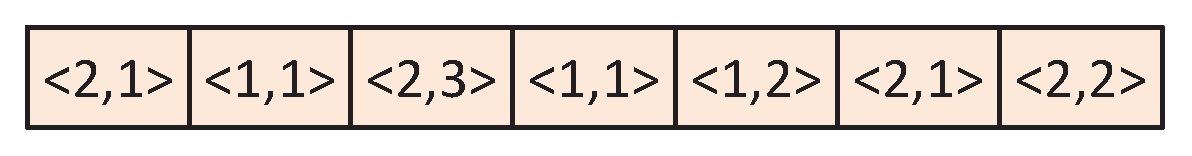
\includegraphics[scale=0.35]{chromo.eps}
	\end{center}
	\vspace{-0.2in}
		\caption{Example of a chromosome}
	\label{fig:chromosome}
\end{figure}
\vspace{-0.1in}

\subsubsection{Initial Population} In a genetic algorithm, the initial population consists of a group of individuals (or chromosomes),
where each of them
%which 
represents a possible solution of the problem. 
A chromosome is composed of several genes that are usually
represented by a random number, or a word or sentence over an
alphabet, or a bit. We use ``integer coding''~\cite{Goldberg} to represent a gene,
i.e. each gene is represented by a pair of non-negative integers. Fig. \ref{fig:chromosome} gives an example of a chromosome. % used in our algorithm.
In a chromosome, any gene $q$ is represented as an integer pair $\langle i,j\rangle$, if  the $q^{th}$ ($q=1\ldots n$) task (in $\Gamma$) is 
assigned to core $\rho_{i,j}$ ($i=1\ldots m$, $j=1\ldots k_i$) (in $\Omega$). The number of genes in a chromosome is equal to $n$.
In  Fig. \ref{fig:chromosome}, the values of $m, k_i, \text{and } n$ are chosen as $2, 3, \text{and } 7$ respectively. 


\subsubsection{Fitness Value} Each chromosome is assigned a \emph{fitness value} which determines the effectiveness of the solution
to the given problem. In our algorithm, the fitness value of a chromosome determines whether the corresponding task allocation 
satisfies the constraints  in Eq. \ref{eq:ilp}, and how effectively 
the task allocation minimizes the
total energy consumption.

Eq. \ref{eq:fitness-p} represents the fitness function of our genetic algorithm, which minimizes the 
overall energy consumption of the system while satisfying the maximum temperature constraints. 
If the allocation strategy corresponding to a chromosome violates Eq. \ref{eq:ilp}, then the penalty of the chromosome is
proportional to the frequency of the core 
%chromosome is penalized
%proportionally to the speed assignment of the core 
which violates  Eq. \ref{eq:ilp} (i.e. $\Lambda \times f_{i,j}$, where
$\Lambda$ is a large integer).
%where the violation happens (Eq. \ref{eq:penalize}). 
Thus, a higher fitness value of a chromosome corresponds to an allocation strategy that results in
a lower total energy consumption without violating the maximum temperature constraints. 


%\begin{equation}\label{eq:fitness}
%Fitness = \kappa * Fitness_{power} ~+~ \nu * Fitness_{temp}
%\end{equation}

\vspace{-0.2in}

\begin{subequations} \label{eq:fitness-p}
	\begin{equation} 
	Fitness = E_{max} - E_{chromo}
	\end{equation}

\vspace{-0.2in}

	\begin{equation}
		E_{max} = P \sum_{i=1}^{m} \sum_{j=1}^{k_i} \Phi_{i,j}(f_{i,j}=f^{max}_{i,j})  %~( \text{when} ~~ f_{i,j}=f^{max}_{i} ) 
	\end{equation}

\vspace{-0.2in}
	
	\begin{equation}  \label{eq:penalize}
	\begin{split}
		&E_{chromo} = P \sum_{i=1}^{m} \sum_{j=1}^{k_i} \Phi^{'}_{i,j}(f_{i,j}) \\
		&\quad %\left( 
		\text{\small where,  } 
		 \Phi^{'}_{i,j}(f_{i,j}) = ~ \left\{ \begin{array}{ll}
		0 & \text{\small If $\rho_{i,j}$ is inactive} \\
		\Phi_{i,j}(f_{i,j}) & \text{\small If Eq. \ref{eq:ilp} is satisfied} \\
		\Lambda \times f_{i,j} & \text{\small Otherwise} \end{array}\right. %\right)
		\end{split}
	\end{equation}
\end{subequations}

\vspace{-0.1in}

\subsubsection{Crossover and Mutation} Crossover and Mutation are two genetic operators which are applied on the chromosomes
to produce new offsprings, hopefully with higher fitness values~\cite{Goldberg}. 
\emph{Top-mate} selection procedure is used to select chromosomes for \emph{two-point crossover} \cite{Goldberg}, where the first chromosome for crossover is selected based on the order of fitness value and the second chromosome is selected randomly from all the chromosomes. In this type of
crossover, the genes between the two randomly chosen points of the selected chromosomes are interchanged with each other. 
An example of a \emph{two-point crossover} %operation 
is given in Fig. \ref{fig:crossover}.

\begin{figure}[h]
	\begin{center}
	%\vspace{-0.1in}
		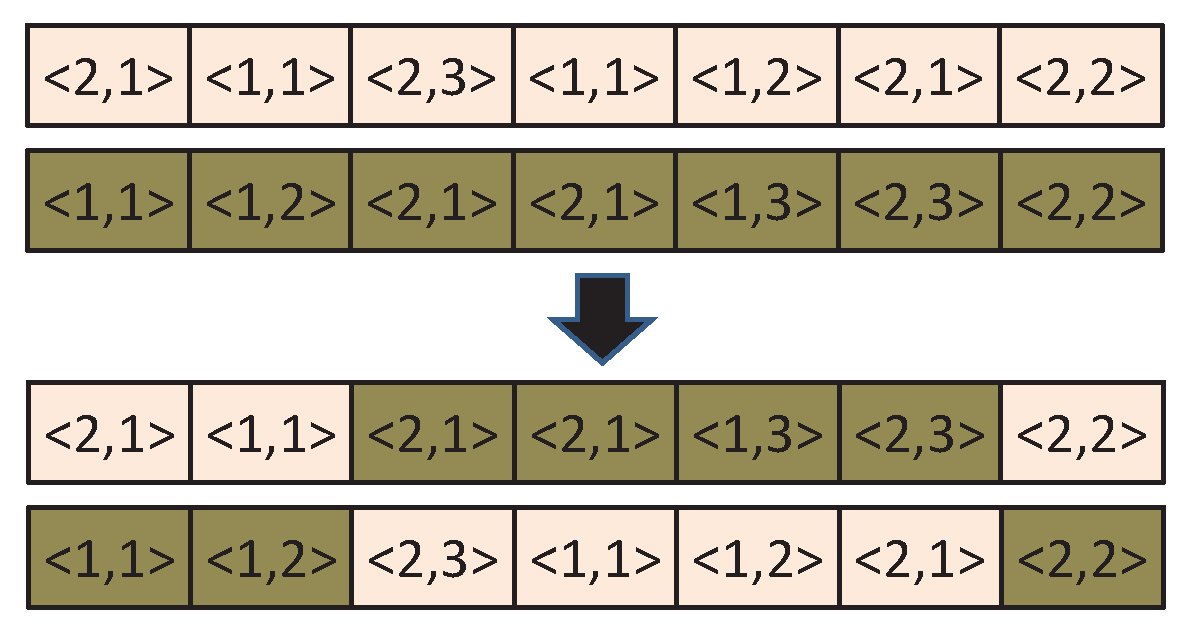
\includegraphics[scale=0.35]{crossover.eps}
	\end{center}
	%\vspace{-0.2in}
		\caption{Example of a two-point crossover}
	\label{fig:crossover}
		%\vspace{-0.1in}
\end{figure}


Mutation %operator 
is applied on the chromosomes to bring diversity in the population. The main objective of mutation
is to avoid losing useful information in the process of evolution \cite{Goldberg}. This also helps to improve the local search performance
of the genetic algorithm. \emph{Two-point mutation} is applied to a randomly selected chromosome. In this operation, the genes between
the two randomly chosen points of the chromosome are assigned new values. Fig. \ref{fig:mutation} gives an example of  \emph{two-point mutation}. % operation.

\begin{figure}[h]
	\begin{center}
	%	\vspace{-0.1in}
		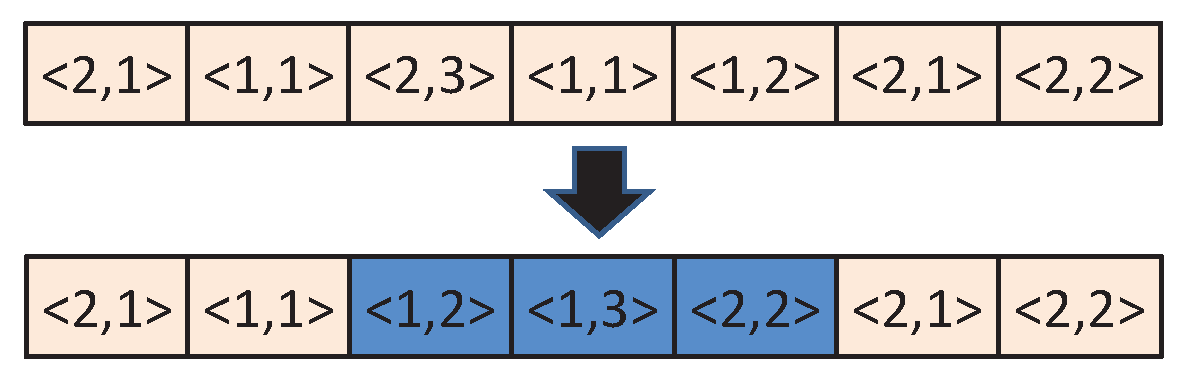
\includegraphics[scale=0.35]{mutation.eps}
	\end{center}
		%\vspace{-0.2in}
		\caption{Example of a two-point mutation}
	\label{fig:mutation}
	%	\vspace{-0.2in}
\end{figure}


\subsubsection{Elitism and Regeneration} To ensure that the best fitness value of the next generation is not worse than that of the current generation, 
a fixed number, MAX$^{elite}$, of best chromosomes are directly copied to the next generation. This operation is called \emph{elitism} \cite{Goldberg}.
The remaining population of the next generation are generated using crossover and mutation operators.


\subsubsection{Termination} The algorithm terminates when a fixed number, MAX$^{gen}$, of generations 
%(denoted by MAX$^{gen}$) 
have been computed, or the algorithm converges, i.e. the best fitness value of the population has not changed for a fixed number
of generations.  

The pseudocode of the Genetic Algorithm (GA) based partitioning approach is given in Algorithm \ref{algo:ga}.

\begin{algorithm} 
\caption{Genetic Algorithm Based Partitioning Approach} \label{algo:ga}
\footnotesize
\begin{algorithmic}[1] 
\STATE Randomly generate the initial population 
\STATE generation $\leftarrow$ 1
\WHILE {generation $\leq$ MAX$^{gen}$}
\STATE Compute fitness of the chromosomes using Eq. \ref{eq:fitness-p}
\STATE Rank the population based on the fitness value
\STATE Copy MAX$^{elite}$ best chromosomes to next generation, ties can be broken randomly
\STATE Generate remaining population using crossover
\STATE Mutate newly generated chromosomes 
\IF {algorithm converged}
\STATE break
\ENDIF
\STATE generation  $\leftarrow$ generation  + 1
\ENDWHILE
\PRINT The total energy consumption, the allocation of tasks to cores, and the active/inactive states of cores that
correspond to the chromosome with the best fitness value (Ties are broken randomly)
\end{algorithmic}
\end{algorithm}

\vspace{-0.1in}



\section{Hybrid Processor Selection Genetic Scheduling Algorithm} %Based Approach}

To find a schedule we combine the above algorithms where first a subset of processors are selected using either \ref{algo:mw} or \ref{algo:bab}, only the cores on these processors are available for scheduling tasks on. An initial population is randomly generated (limited to valid schedules). Feed the initial population into algorithm \ref{algo:ga}.

\begin{algorithm} 
\caption{Hybrid Processor Selection Genetic Scheduling Algorithm} \label{algo:hypsgsa}
\footnotesize
\begin{algorithmic}[1] 
\STATE Get a set of processors from a selection algorithm, \ref{algo:mw} or \ref{algo:bab}
\STATE Randomly generate a population of valid schedules on cores from selected processors
\STATE Call Algorithm \ref{algo:ga} on this initial population
\end{algorithmic}
\end{algorithm}
\vspace{-0.2in}



\bibliography{rtss2}
\bibliographystyle{ieeetr}

%
%\begin{thebibliography}{00}
%\end{thebibliography}

\end{document}